\chapter{Nuclear Medicine Imaging}
\label{ch:nuclear_medicine}

% Chapter-opening illustrated modality infographic.
\begin{center}
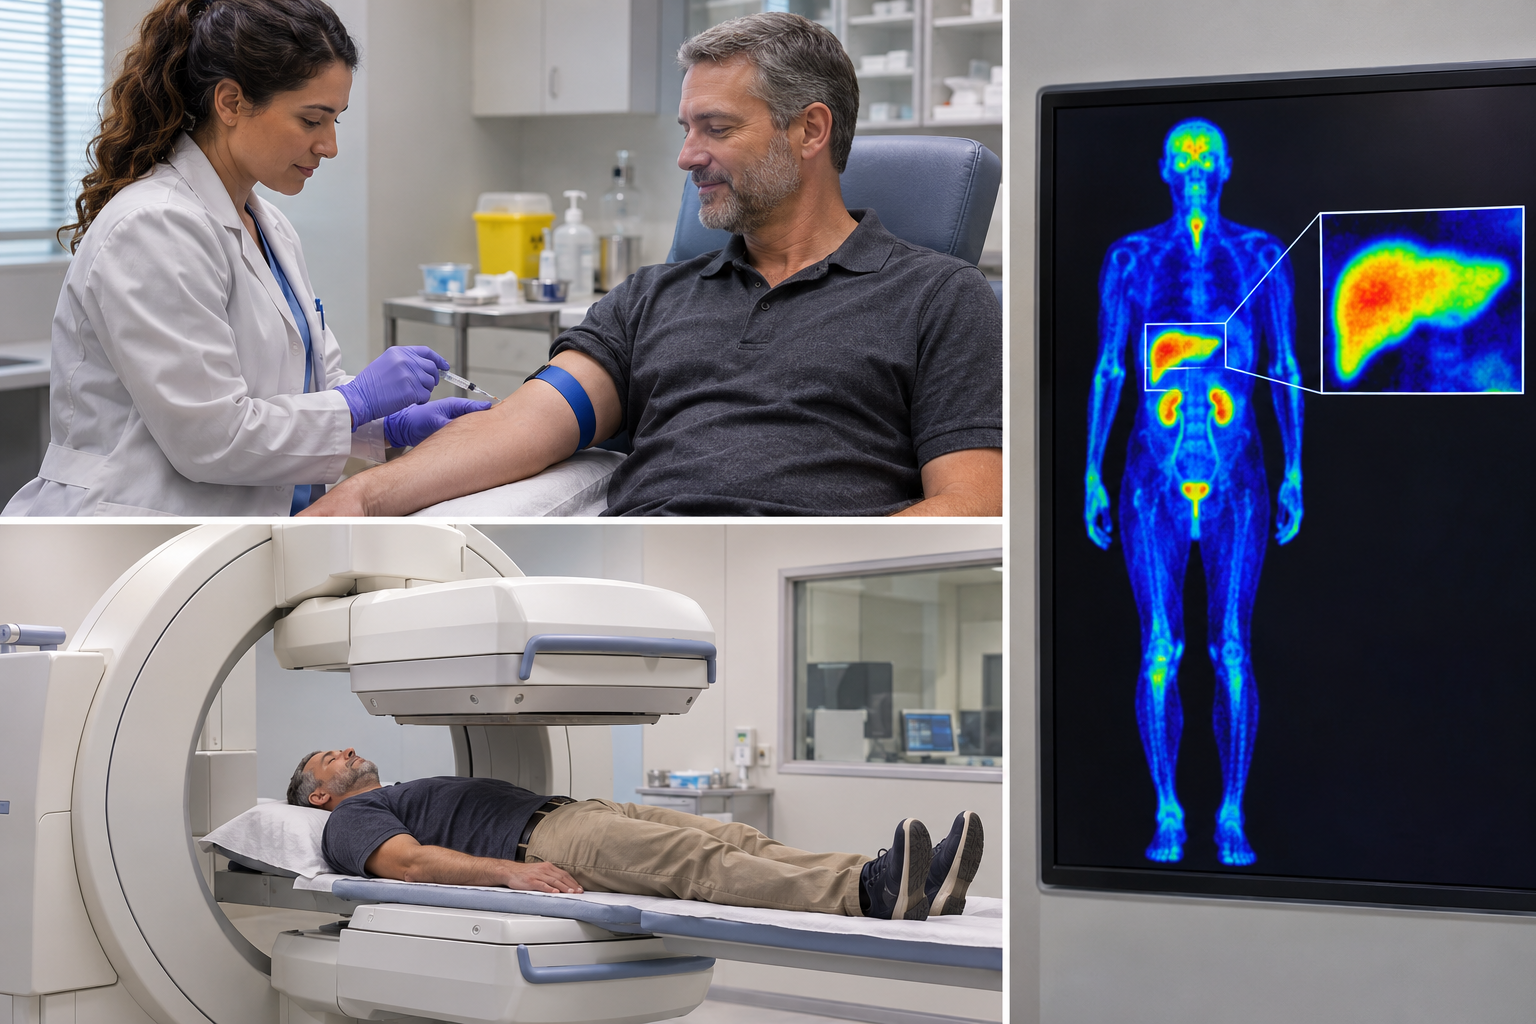
\includegraphics[width=\textwidth,keepaspectratio]{modalities/infographics/nuclear_medicine_realistic.png}
\end{center}
\begin{center}\footnotesize Radiopharmaceutical distribution reflects a tracer-specific biological process, and a gamma camera detects emitted photons to map that activity. AI-generated illustration; scan panel is not a patient study.\end{center}

\section{Overview}
Nuclear medicine is a diagnostic imaging discipline that uses radiopharmaceuticals to investigate physiological function, metabolism, tissue perfusion, receptor expression, and molecular processes within the human body.

Unlike CT and conventional MRI, which primarily visualize anatomical structures, nuclear medicine can reveal functional and molecular abnormalities before substantial anatomical changes become apparent.

Principal diagnostic modalities include planar scintigraphy, single-photon emission computed tomography (SPECT), positron emission tomography (PET), hybrid SPECT/CT, hybrid PET/CT, and hybrid PET/MRI. This chapter covers diseases and conditions for which nuclear medicine provides established or supplementary diagnostic information. Therapeutic nuclear medicine is excluded.

The 195 entries form a preliminary catalogue of nuclear medicine applications, including diagnosis, staging, localization, functional assessment, and treatment monitoring. Some entries overlap or represent historical or nonroutine applications; individual indications and radiopharmaceutical assignments require validation against clinical guidelines.

\section{Where nuclear medicine is used}
The following catalogue groups applications by disease category. Findings should be interpreted in the context of the administered radiopharmaceutical, acquisition protocol, and clinical question.

\subsection{Neurological and neurodegenerative diseases}
\begin{enumerate}[leftmargin=*,itemsep=0.45em,topsep=0.4em]
\item \textbf{Alzheimer disease.} Useful imaging findings include: Temporoparietal and posterior cingulate hypometabolism. Radiopharmaceutical: ¹⁸F-FDG.
\item \textbf{Alzheimer-associated amyloid pathology.} Useful imaging findings include: Increased cortical amyloid tracer retention. Radiopharmaceutical: ¹⁸F-Florbetapir, ¹⁸F-Flutemetamol.
\item \textbf{Alzheimer-associated tau pathology.} Useful imaging findings include: Increased regional tau tracer retention. Radiopharmaceutical: ¹⁸F-Flortaucipir.
\item \textbf{Cerebral circulatory arrest.} Useful imaging findings include: Absence of intracranial perfusion on a protocol-based ancillary study. Radiopharmaceutical: ⁹⁹ᵐTc-HMPAO.
\item \textbf{Cerebral ischemia.} Useful imaging findings include: Regional reduction in cerebral perfusion. Radiopharmaceutical: ⁹⁹ᵐTc-ECD.
\item \textbf{Corticobasal syndrome.} Useful imaging findings include: Asymmetric cortical and subcortical hypometabolism. Radiopharmaceutical: ¹⁸F-FDG.
\item \textbf{Dementia with Lewy bodies.} Useful imaging findings include: Occipital hypometabolism. Radiopharmaceutical: ¹⁸F-FDG.
\item \textbf{Focal epilepsy.} Useful imaging findings include: Increased ictal regional perfusion. Radiopharmaceutical: ⁹⁹ᵐTc-HMPAO.
\item \textbf{Frontotemporal dementia.} Useful imaging findings include: Frontal and anterior temporal hypometabolism. Radiopharmaceutical: ¹⁸F-FDG.
\item \textbf{Huntington disease.} Useful imaging findings include: Striatal hypometabolism. Radiopharmaceutical: ¹⁸F-FDG.
\item \textbf{Multiple system atrophy.} Useful imaging findings include: Reduced striatal dopamine transporter binding. Radiopharmaceutical: ¹²³I-Ioflupane.
\item \textbf{Parkinson disease.} Useful imaging findings include: Reduced striatal dopamine transporter binding. Radiopharmaceutical: ¹²³I-Ioflupane.
\item \textbf{Progressive supranuclear palsy.} Useful imaging findings include: Frontal and midbrain hypometabolism. Radiopharmaceutical: ¹⁸F-FDG.
\item \textbf{Temporal lobe epilepsy.} Useful imaging findings include: Interictal temporal hypometabolism. Radiopharmaceutical: ¹⁸F-FDG.
\item \textbf{Vascular dementia.} Useful imaging findings include: Regional metabolic or perfusion defects. Radiopharmaceutical: ¹⁸F-FDG.
\end{enumerate}
Dopamine transporter imaging cannot reliably distinguish Parkinson disease from several atypical degenerative parkinsonian syndromes.
In suspected death by neurologic criteria, radionuclide cerebral perfusion imaging is an ancillary test performed under applicable protocols; absent intracranial perfusion does not by itself establish the clinical diagnosis.

\subsection{Brain tumors}
\begin{enumerate}[leftmargin=*,itemsep=0.45em,topsep=0.4em]
\item \textbf{Astrocytoma.} Useful imaging findings include: Variable amino acid uptake. Radiopharmaceutical: ¹⁸F-FET.
\item \textbf{Brain metastases.} Useful imaging findings include: Variable amino acid tracer uptake. Radiopharmaceutical: ¹⁸F-FET.
\item \textbf{Glioblastoma.} Useful imaging findings include: Increased amino acid tracer uptake. Radiopharmaceutical: ¹⁸F-FET.
\item \textbf{Meningioma.} Useful imaging findings include: Increased somatostatin receptor expression. Radiopharmaceutical: ⁶⁸Ga-DOTATATE.
\item \textbf{Oligodendroglioma.} Useful imaging findings include: Variable or increased amino acid uptake. Radiopharmaceutical: ¹¹C-Methionine.
\item \textbf{Primary CNS lymphoma.} Useful imaging findings include: Markedly increased glucose metabolism. Radiopharmaceutical: ¹⁸F-FDG.
\item \textbf{Radiation necrosis.} Useful imaging findings include: Generally lower amino acid uptake than recurrent tumor, with overlap. Radiopharmaceutical: ¹⁸F-FET.
\item \textbf{Recurrent glioma.} Useful imaging findings include: Increased uptake within viable tumor tissue. Radiopharmaceutical: ¹⁸F-FET.
\end{enumerate}

\subsection{Cardiovascular diseases}
\begin{enumerate}[leftmargin=*,itemsep=0.45em,topsep=0.4em]
\item \textbf{Aortitis.} Useful imaging findings include: Increased aortic wall uptake. Radiopharmaceutical: ¹⁸F-FDG.
\item \textbf{Cardiac device infection.} Useful imaging findings include: Increased uptake surrounding implanted devices. Radiopharmaceutical: ¹⁸F-FDG.
\item \textbf{Cardiac sarcoidosis.} Useful imaging findings include: Focal myocardial inflammatory uptake. Radiopharmaceutical: ¹⁸F-FDG.
\item \textbf{Coronary artery disease.} Useful imaging findings include: Stress-induced myocardial perfusion defects. Radiopharmaceutical: ⁹⁹ᵐTc-Sestamibi.
\item \textbf{Coronary microvascular dysfunction.} Useful imaging findings include: Reduced myocardial flow reserve. Radiopharmaceutical: ⁸²Rb, ¹³N-Ammonia.
\item \textbf{Dilated cardiomyopathy.} Useful imaging findings include: Reduced ventricular ejection fraction; chamber size requires anatomical imaging correlation. Radiopharmaceutical: ⁹⁹ᵐTc-labeled RBCs (equilibrium radionuclide ventriculography).
\item \textbf{Giant cell arteritis.} Useful imaging findings include: Increased arterial wall metabolic activity. Radiopharmaceutical: ¹⁸F-FDG.
\item \textbf{Hibernating myocardium.} Useful imaging findings include: Reduced perfusion with preserved glucose metabolism (perfusion--metabolism mismatch). Radiopharmaceutical: ¹⁸F-FDG with paired perfusion imaging (e.g., ⁸²Rb or ¹³N-ammonia PET).
\item \textbf{Ischemic cardiomyopathy.} Useful imaging findings include: Regional perfusion and functional abnormalities. Radiopharmaceutical: ⁹⁹ᵐTc-Sestamibi.
\item \textbf{Myocardial ischemia.} Useful imaging findings include: Reversible myocardial perfusion defect. Radiopharmaceutical: ⁹⁹ᵐTc-Tetrofosmin.
\item \textbf{Previous myocardial infarction.} Useful imaging findings include: Fixed myocardial perfusion defect. Radiopharmaceutical: ⁹⁹ᵐTc-Sestamibi.
\item \textbf{Prosthetic valve endocarditis.} Useful imaging findings include: Abnormal periprosthetic tracer uptake. Radiopharmaceutical: ¹⁸F-FDG.
\item \textbf{Takayasu arteritis.} Useful imaging findings include: Increased uptake in inflamed large arteries. Radiopharmaceutical: ¹⁸F-FDG.
\item \textbf{Transthyretin cardiac amyloidosis.} Useful imaging findings include: Myocardial bone-tracer uptake assessed using validated visual and SPECT criteria. Radiopharmaceutical: ⁹⁹ᵐTc-PYP, DPD or HMDP.
\item \textbf{Vascular graft infection.} Useful imaging findings include: Abnormal uptake surrounding vascular grafts. Radiopharmaceutical: ¹⁸F-FDG.
\end{enumerate}
Bone-tracer uptake supports ATTR cardiac amyloidosis only in the appropriate clinical context. Evaluation for a monoclonal protein is required to avoid misclassifying AL amyloidosis; uptake alone is not diagnostic.

\subsection{Pulmonary diseases}
\begin{enumerate}[leftmargin=*,itemsep=0.45em,topsep=0.4em]
\item \textbf{Acute pulmonary embolism.} Useful imaging findings include: Segmental ventilation--perfusion mismatch; perfusion-only imaging may be used in selected protocols. Radiopharmaceutical: ⁹⁹ᵐTc-MAA plus a ventilation agent (e.g., ⁹⁹ᵐTc-Technegas or aerosol).
\item \textbf{Bronchogenic carcinoma.} Useful imaging findings include: Increased tumor glucose metabolism. Radiopharmaceutical: ¹⁸F-FDG.
\item \textbf{Chronic obstructive pulmonary disease.} Useful imaging findings include: Heterogeneous ventilation and perfusion. Radiopharmaceutical: ⁹⁹ᵐTc-MAA, Technegas.
\item \textbf{Chronic thromboembolic pulmonary hypertension.} Useful imaging findings include: Persistent mismatched ventilation--perfusion defects. Radiopharmaceutical: ⁹⁹ᵐTc-MAA plus a ventilation agent (e.g., ⁹⁹ᵐTc-Technegas or aerosol).
\item \textbf{Malignant pleural mesothelioma.} Useful imaging findings include: Increased pleural metabolic activity. Radiopharmaceutical: ¹⁸F-FDG.
\item \textbf{Pulmonary emphysema.} Useful imaging findings include: Regional ventilation and perfusion abnormalities. Radiopharmaceutical: ⁹⁹ᵐTc-MAA.
\item \textbf{Pulmonary fibrosis (selected preoperative regional function assessment).} Useful imaging findings include: Regional perfusion contribution to lung function; this study does not diagnose pulmonary fibrosis. Radiopharmaceutical: ⁹⁹ᵐTc-MAA.
\item \textbf{Pulmonary metastases.} Useful imaging findings include: Variable focal metabolic uptake. Radiopharmaceutical: ¹⁸F-FDG.
\item \textbf{Pulmonary sarcoidosis.} Useful imaging findings include: Increased metabolic activity in active inflammatory lesions. Radiopharmaceutical: ¹⁸F-FDG.
\item \textbf{Right-to-left pulmonary shunt (including selected assessment in pulmonary arteriovenous malformation).} Useful imaging findings include: Extrapulmonary activity used to detect or quantify right-to-left shunting; does not localize a malformation. Radiopharmaceutical: ⁹⁹ᵐTc-MAA.
\end{enumerate}

\subsection{Thyroid and parathyroid diseases}
\begin{enumerate}[leftmargin=*,itemsep=0.45em,topsep=0.4em]
\item \textbf{Autonomous thyroid nodule.} Useful imaging findings include: Focal increased tracer uptake. Radiopharmaceutical: ¹²³I.
\item \textbf{Congenital thyroid dysgenesis.} Useful imaging findings include: Absent or ectopic thyroid uptake. Radiopharmaceutical: ⁹⁹ᵐTc-Pertechnetate.
\item \textbf{Ectopic parathyroid adenoma.} Useful imaging findings include: Focal uptake at an abnormal anatomical location. Radiopharmaceutical: ¹⁸F-Fluorocholine.
\item \textbf{Ectopic thyroid tissue.} Useful imaging findings include: Tracer uptake outside the normal thyroid location. Radiopharmaceutical: ⁹⁹ᵐTc-Pertechnetate.
\item \textbf{Follicular thyroid carcinoma.} Useful imaging findings include: Possible radioiodine-avid metastatic lesions. Radiopharmaceutical: ¹²³I, ¹³¹I.
\item \textbf{Graves disease.} Useful imaging findings include: Diffusely increased thyroid uptake. Radiopharmaceutical: ¹²³I, ⁹⁹ᵐTc-Pertechnetate.
\item \textbf{Hashimoto thyroiditis.} Useful imaging findings include: Variable or heterogeneous uptake. Radiopharmaceutical: ¹²³I.
\item \textbf{Painless thyroiditis.} Useful imaging findings include: Reduced thyroid uptake. Radiopharmaceutical: ¹²³I.
\item \textbf{Papillary thyroid carcinoma.} Useful imaging findings include: Possible radioiodine uptake in residual or metastatic disease. Radiopharmaceutical: ¹²³I, ¹³¹I.
\item \textbf{Parathyroid adenoma.} Useful imaging findings include: Persistent focal tracer retention. Radiopharmaceutical: ⁹⁹ᵐTc-Sestamibi.
\item \textbf{Parathyroid hyperplasia.} Useful imaging findings include: Uptake in multiple enlarged glands. Radiopharmaceutical: ⁹⁹ᵐTc-Sestamibi.
\item \textbf{Radioiodine-refractory thyroid carcinoma.} Useful imaging findings include: Increased glucose metabolism in some lesions. Radiopharmaceutical: ¹⁸F-FDG.
\item \textbf{Subacute thyroiditis.} Useful imaging findings include: Markedly reduced thyroid uptake. Radiopharmaceutical: ¹²³I.
\item \textbf{Toxic multinodular goiter.} Useful imaging findings include: Heterogeneous increased thyroid uptake. Radiopharmaceutical: ¹²³I.
\item \textbf{Toxic thyroid adenoma.} Useful imaging findings include: Focal increased uptake with suppressed surrounding tissue. Radiopharmaceutical: ⁹⁹ᵐTc-Pertechnetate.
\end{enumerate}

\subsection{Bones and skeletal diseases}
\begin{enumerate}[leftmargin=*,itemsep=0.45em,topsep=0.4em]
\item \textbf{Acute osteomyelitis.} Useful imaging findings include: Increased perfusion, blood-pool and delayed uptake. Radiopharmaceutical: ⁹⁹ᵐTc-MDP.
\item \textbf{Breast cancer bone metastases.} Useful imaging findings include: Increased skeletal uptake or metabolism. Radiopharmaceutical: ⁹⁹ᵐTc-MDP, ¹⁸F-FDG.
\item \textbf{Chondrosarcoma.} Useful imaging findings include: Variable metabolic uptake. Radiopharmaceutical: ¹⁸F-FDG.
\item \textbf{Chronic osteomyelitis.} Useful imaging findings include: Abnormal osseous metabolic or inflammatory uptake. Radiopharmaceutical: ¹⁸F-FDG.
\item \textbf{Complex regional pain syndrome.} Useful imaging findings include: Variable regional periarticular uptake. Radiopharmaceutical: ⁹⁹ᵐTc-MDP.
\item \textbf{Ewing sarcoma.} Useful imaging findings include: Increased tumor glucose metabolism. Radiopharmaceutical: ¹⁸F-FDG.
\item \textbf{Fibrous dysplasia.} Useful imaging findings include: Increased regional skeletal uptake. Radiopharmaceutical: ⁹⁹ᵐTc-MDP.
\item \textbf{Heterotopic ossification.} Useful imaging findings include: Increased extraosseous bone-tracer uptake. Radiopharmaceutical: ⁹⁹ᵐTc-MDP.
\item \textbf{Hypertrophic osteoarthropathy.} Useful imaging findings include: Symmetric linear periosteal uptake. Radiopharmaceutical: ⁹⁹ᵐTc-MDP.
\item \textbf{Multiple myeloma.} Useful imaging findings include: Metabolically active marrow or skeletal lesions. Radiopharmaceutical: ¹⁸F-FDG.
\item \textbf{Occult fracture.} Useful imaging findings include: Increased uptake at fracture site. Radiopharmaceutical: ⁹⁹ᵐTc-MDP.
\item \textbf{Osteoblastic bone metastases.} Useful imaging findings include: Multifocal increased skeletal uptake. Radiopharmaceutical: ⁹⁹ᵐTc-MDP.
\item \textbf{Osteoblastoma.} Useful imaging findings include: Increased focal skeletal uptake. Radiopharmaceutical: ⁹⁹ᵐTc-MDP.
\item \textbf{Osteoid osteoma.} Useful imaging findings include: Intense focal uptake. Radiopharmaceutical: ⁹⁹ᵐTc-MDP.
\item \textbf{Osteonecrosis.} Useful imaging findings include: Reduced early perfusion or variable reparative uptake. Radiopharmaceutical: ⁹⁹ᵐTc-MDP.
\item \textbf{Osteosarcoma.} Useful imaging findings include: Increased tumor metabolic activity. Radiopharmaceutical: ¹⁸F-FDG.
\item \textbf{Paget disease of bone.} Useful imaging findings include: Intense uptake involving affected bone. Radiopharmaceutical: ⁹⁹ᵐTc-MDP.
\item \textbf{Prostate cancer bone metastases.} Useful imaging findings include: Increased osteoblastic activity. Radiopharmaceutical: ⁹⁹ᵐTc-MDP, ¹⁸F-NaF.
\item \textbf{Stress fracture.} Useful imaging findings include: Focal increased skeletal uptake. Radiopharmaceutical: ⁹⁹ᵐTc-MDP.
\item \textbf{Vertebral compression fracture.} Useful imaging findings include: Increased uptake in metabolically active fractures. Radiopharmaceutical: ⁹⁹ᵐTc-MDP.
\end{enumerate}
Conventional bone scintigraphy is less sensitive for purely osteolytic lesions, including many multiple myeloma lesions.

\subsection{Joint and prosthetic disorders}
\begin{enumerate}[leftmargin=*,itemsep=0.45em,topsep=0.4em]
\item \textbf{Aseptic prosthetic loosening.} Useful imaging findings include: Increased bone turnover at prosthetic interfaces. Radiopharmaceutical: ⁹⁹ᵐTc-MDP.
\item \textbf{Osteoarthritis.} Useful imaging findings include: Increased periarticular bone turnover. Radiopharmaceutical: ⁹⁹ᵐTc-MDP.
\item \textbf{Painful hip arthroplasty.} Useful imaging findings include: Abnormal periprosthetic tracer uptake. Radiopharmaceutical: ⁹⁹ᵐTc-MDP.
\item \textbf{Painful knee arthroplasty.} Useful imaging findings include: Abnormal regional bone turnover. Radiopharmaceutical: ⁹⁹ᵐTc-MDP.
\item \textbf{Prosthetic joint infection.} Useful imaging findings include: Abnormal periprosthetic leukocyte accumulation, interpreted with the clinical context and complementary imaging when indicated. Radiopharmaceutical: ¹¹¹In-Oxine leukocytes.
\item \textbf{Rheumatoid arthritis.} Useful imaging findings include: Increased inflammatory joint uptake. Radiopharmaceutical: ¹⁸F-FDG.
\item \textbf{Sacroiliac inflammation.} Useful imaging findings include: Variable increased metabolic activity. Radiopharmaceutical: ¹⁸F-FDG.
\item \textbf{Septic arthritis.} Useful imaging findings include: Increased inflammatory tracer accumulation. Radiopharmaceutical: ¹⁸F-FDG, labeled leukocytes.
\end{enumerate}

\subsection{Liver and biliary diseases}
\begin{enumerate}[leftmargin=*,itemsep=0.45em,topsep=0.4em]
\item \textbf{Acute cholecystitis.} Useful imaging findings include: Nonvisualization of the gallbladder under appropriate protocol. Radiopharmaceutical: ⁹⁹ᵐTc-Mebrofenin.
\item \textbf{Bile leak.} Useful imaging findings include: Extraluminal accumulation of biliary tracer. Radiopharmaceutical: ⁹⁹ᵐTc-Mebrofenin.
\item \textbf{Biliary atresia.} Useful imaging findings include: Absent intestinal tracer excretion after an appropriate protocol; this is not specific and may also occur with severe hepatocellular dysfunction. Radiopharmaceutical: ⁹⁹ᵐTc-Mebrofenin.
\item \textbf{Biliary obstruction.} Useful imaging findings include: Delayed or absent tracer passage into the intestine. Radiopharmaceutical: ⁹⁹ᵐTc-Mebrofenin.
\item \textbf{Cholangiocarcinoma.} Useful imaging findings include: Increased metabolic uptake in many tumors. Radiopharmaceutical: ¹⁸F-FDG.
\item \textbf{Chronic cholecystitis.} Useful imaging findings include: Delayed gallbladder visualization or abnormal emptying. Radiopharmaceutical: ⁹⁹ᵐTc-Disofenin.
\item \textbf{Focal nodular hyperplasia.} Useful imaging findings include: Preserved or increased reticuloendothelial tracer uptake in some lesions. Radiopharmaceutical: ⁹⁹ᵐTc-Sulfur colloid.
\item \textbf{Functional gallbladder disorder.} Useful imaging findings include: Reduced gallbladder ejection fraction. Radiopharmaceutical: ⁹⁹ᵐTc-Mebrofenin.
\item \textbf{Hepatic hemangioma.} Useful imaging findings include: Delayed blood-pool accumulation. Radiopharmaceutical: ⁹⁹ᵐTc-labeled RBCs.
\item \textbf{Hepatic metastases.} Useful imaging findings include: Focal abnormal metabolic or receptor-specific uptake. Radiopharmaceutical: ¹⁸F-FDG, ⁶⁸Ga-DOTATATE.
\item \textbf{Hepatocellular carcinoma.} Useful imaging findings include: Variable glucose metabolism. Radiopharmaceutical: ¹⁸F-FDG.
\item \textbf{Neonatal hepatitis.} Useful imaging findings include: Impaired hepatic uptake and excretion. Radiopharmaceutical: ⁹⁹ᵐTc-Mebrofenin.
\end{enumerate}

\subsection{Gastrointestinal diseases}
\begin{enumerate}[leftmargin=*,itemsep=0.45em,topsep=0.4em]
\item \textbf{Active gastrointestinal bleeding.} Useful imaging findings include: Extravascular accumulation and movement of labeled blood. Radiopharmaceutical: ⁹⁹ᵐTc-labeled RBCs.
\item \textbf{Chronic intestinal dysmotility.} Useful imaging findings include: Abnormal gastrointestinal transit. Radiopharmaceutical: Radiolabeled meals.
\item \textbf{Colonic slow-transit constipation.} Useful imaging findings include: Delayed colonic tracer progression. Radiopharmaceutical: ¹¹¹In-labeled tracer.
\item \textbf{Crohn disease.} Useful imaging findings include: Increased inflammatory bowel uptake. Radiopharmaceutical: ¹⁸F-FDG.
\item \textbf{Esophageal motility disorder.} Useful imaging findings include: Delayed esophageal tracer transit. Radiopharmaceutical: ⁹⁹ᵐTc-labeled liquid.
\item \textbf{Gastroparesis.} Useful imaging findings include: Delayed gastric emptying. Radiopharmaceutical: ⁹⁹ᵐTc-Sulfur colloid-labeled meal.
\item \textbf{Meckel diverticulum.} Useful imaging findings include: Ectopic gastric mucosal tracer uptake. Radiopharmaceutical: ⁹⁹ᵐTc-Pertechnetate.
\item \textbf{Protein-losing enteropathy.} Useful imaging findings include: Abnormal leakage of labeled protein into the bowel. Radiopharmaceutical: ⁹⁹ᵐTc-Human serum albumin.
\item \textbf{Rapid gastric emptying.} Useful imaging findings include: Accelerated gastric tracer clearance. Radiopharmaceutical: ⁹⁹ᵐTc-Sulfur colloid-labeled meal.
\item \textbf{Ulcerative colitis.} Useful imaging findings include: Increased colonic inflammatory uptake. Radiopharmaceutical: ¹⁸F-FDG.
\end{enumerate}

\subsection{Renal and urinary tract diseases}
\begin{enumerate}[leftmargin=*,itemsep=0.45em,topsep=0.4em]
\item \textbf{Acute pyelonephritis.} Useful imaging findings include: Focal renal cortical uptake defects. Radiopharmaceutical: ⁹⁹ᵐTc-DMSA.
\item \textbf{Ectopic kidney.} Useful imaging findings include: Renal tracer uptake at an abnormal location. Radiopharmaceutical: ⁹⁹ᵐTc-DMSA.
\item \textbf{Horseshoe kidney.} Useful imaging findings include: Abnormal renal configuration. Radiopharmaceutical: ⁹⁹ᵐTc-DMSA.
\item \textbf{Hydronephrosis.} Useful imaging findings include: Collecting-system retention with variable drainage. Radiopharmaceutical: ⁹⁹ᵐTc-MAG3.
\item \textbf{Obstructive uropathy.} Useful imaging findings include: Impaired urinary tracer clearance. Radiopharmaceutical: ⁹⁹ᵐTc-MAG3.
\item \textbf{Reflux nephropathy.} Useful imaging findings include: Cortical defects and impaired differential function. Radiopharmaceutical: ⁹⁹ᵐTc-DMSA.
\item \textbf{Renal artery stenosis.} Useful imaging findings include: Abnormal renal perfusion or captopril renographic response. Radiopharmaceutical: ⁹⁹ᵐTc-DTPA.
\item \textbf{Renal cortical scarring.} Useful imaging findings include: Persistent cortical tracer defects. Radiopharmaceutical: ⁹⁹ᵐTc-DMSA.
\item \textbf{Renal dysplasia.} Useful imaging findings include: Reduced or abnormal cortical tracer distribution. Radiopharmaceutical: ⁹⁹ᵐTc-DMSA.
\item \textbf{Renal infarction.} Useful imaging findings include: Regional absence of cortical uptake. Radiopharmaceutical: ⁹⁹ᵐTc-DMSA.
\item \textbf{Renal transplant dysfunction.} Useful imaging findings include: Abnormal perfusion, uptake or excretion. Radiopharmaceutical: ⁹⁹ᵐTc-MAG3.
\item \textbf{Renal transplant urinary leak.} Useful imaging findings include: Extraluminal urinary tracer accumulation. Radiopharmaceutical: ⁹⁹ᵐTc-MAG3.
\item \textbf{Renovascular hypertension.} Useful imaging findings include: Altered renal function following ACE inhibition. Radiopharmaceutical: ⁹⁹ᵐTc-MAG3.
\item \textbf{Ureteropelvic junction obstruction.} Useful imaging findings include: Delayed tracer drainage despite diuretic administration. Radiopharmaceutical: ⁹⁹ᵐTc-MAG3.
\item \textbf{Vesicoureteral reflux.} Useful imaging findings include: Retrograde tracer movement into ureters. Radiopharmaceutical: Radionuclide cystography tracer.
\end{enumerate}

\subsection{Neuroendocrine and adrenal diseases}
\begin{enumerate}[leftmargin=*,itemsep=0.45em,topsep=0.4em]
\item \textbf{Adrenocortical carcinoma.} Useful imaging findings include: Increased glucose metabolism in many tumors. Radiopharmaceutical: ¹⁸F-FDG.
\item \textbf{Bronchial carcinoid.} Useful imaging findings include: Increased somatostatin receptor expression. Radiopharmaceutical: ⁶⁸Ga-DOTATATE.
\item \textbf{Gastrinoma.} Useful imaging findings include: Increased somatostatin receptor uptake. Radiopharmaceutical: ⁶⁸Ga-DOTATATE.
\item \textbf{Gastroenteropancreatic neuroendocrine tumor.} Useful imaging findings include: Increased somatostatin receptor tracer uptake. Radiopharmaceutical: ⁶⁸Ga-DOTATATE.
\item \textbf{Insulinoma.} Useful imaging findings include: Variable GLP-1 receptor or somatostatin receptor uptake. Radiopharmaceutical: Radiolabeled exendin.
\item \textbf{Medullary thyroid carcinoma.} Useful imaging findings include: Variable amino acid or receptor-specific uptake. Radiopharmaceutical: ¹⁸F-FDOPA.
\item \textbf{Merkel cell carcinoma.} Useful imaging findings include: Increased glucose metabolism. Radiopharmaceutical: ¹⁸F-FDG.
\item \textbf{Neuroblastoma.} Useful imaging findings include: Increased norepinephrine transporter-related uptake. Radiopharmaceutical: ¹²³I-MIBG.
\item \textbf{Pancreatic neuroendocrine tumor.} Useful imaging findings include: Increased receptor-specific uptake. Radiopharmaceutical: ⁶⁸Ga-DOTATATE.
\item \textbf{Paraganglioma.} Useful imaging findings include: Increased somatostatin receptor expression. Radiopharmaceutical: ⁶⁸Ga-DOTATATE.
\item \textbf{Pheochromocytoma.} Useful imaging findings include: Increased catecholamine-related or receptor-specific uptake. Radiopharmaceutical: ¹²³I-MIBG, ⁶⁸Ga-DOTATATE.
\item \textbf{Small bowel neuroendocrine tumor.} Useful imaging findings include: Receptor-positive primary and metastatic lesions. Radiopharmaceutical: ⁶⁸Ga-DOTATATE.
\end{enumerate}

\subsection{Hematological malignancies}
\begin{enumerate}[leftmargin=*,itemsep=0.45em,topsep=0.4em]
\item \textbf{Burkitt lymphoma.} Useful imaging findings include: Intense metabolic uptake. Radiopharmaceutical: ¹⁸F-FDG.
\item \textbf{Diffuse large B-cell lymphoma.} Useful imaging findings include: Markedly increased metabolic activity. Radiopharmaceutical: ¹⁸F-FDG.
\item \textbf{Extramedullary plasmacytoma.} Useful imaging findings include: Hypermetabolic soft-tissue lesion. Radiopharmaceutical: ¹⁸F-FDG.
\item \textbf{Follicular lymphoma.} Useful imaging findings include: Increased nodal metabolic activity. Radiopharmaceutical: ¹⁸F-FDG.
\item \textbf{Hodgkin lymphoma.} Useful imaging findings include: Hypermetabolic lymph nodes and extranodal lesions. Radiopharmaceutical: ¹⁸F-FDG.
\item \textbf{Mantle cell lymphoma.} Useful imaging findings include: Variable or increased metabolic uptake. Radiopharmaceutical: ¹⁸F-FDG.
\item \textbf{Marginal zone lymphoma.} Useful imaging findings include: Variable metabolic activity. Radiopharmaceutical: ¹⁸F-FDG.
\item \textbf{Multiple myeloma.} Useful imaging findings include: Focal or diffuse metabolically active marrow lesions. Radiopharmaceutical: ¹⁸F-FDG.
\item \textbf{Peripheral T-cell lymphoma.} Useful imaging findings include: Increased metabolic uptake. Radiopharmaceutical: ¹⁸F-FDG.
\item \textbf{Primary mediastinal B-cell lymphoma.} Useful imaging findings include: Increased mediastinal metabolic activity. Radiopharmaceutical: ¹⁸F-FDG.
\item \textbf{Richter transformation.} Useful imaging findings include: Increased metabolic activity in suspicious lesions. Radiopharmaceutical: ¹⁸F-FDG.
\item \textbf{Solitary plasmacytoma.} Useful imaging findings include: Focal metabolically active lesion. Radiopharmaceutical: ¹⁸F-FDG.
\end{enumerate}

\subsection{Solid malignant tumors}
Nuclear medicine is extensively used in oncology for tumor staging, treatment response assessment, recurrence detection, and selection of targeted therapies.
\begin{enumerate}[leftmargin=*,itemsep=0.45em,topsep=0.4em]
\item \textbf{Bladder carcinoma.} Useful imaging findings include: Increased tumor or metastatic metabolic activity. Radiopharmaceutical: ¹⁸F-FDG.
\item \textbf{Breast carcinoma.} Useful imaging findings include: Variable increased tumor metabolism. Radiopharmaceutical: ¹⁸F-FDG.
\item \textbf{Cancer of unknown primary.} Useful imaging findings include: Abnormal metabolic foci suggesting primary tumor. Radiopharmaceutical: ¹⁸F-FDG.
\item \textbf{Cervical carcinoma.} Useful imaging findings include: Increased primary and metastatic tumor uptake. Radiopharmaceutical: ¹⁸F-FDG.
\item \textbf{Colorectal carcinoma.} Useful imaging findings include: Increased metabolic activity. Radiopharmaceutical: ¹⁸F-FDG.
\item \textbf{Endometrial carcinoma.} Useful imaging findings include: Hypermetabolic uterine or metastatic lesions. Radiopharmaceutical: ¹⁸F-FDG.
\item \textbf{Esophageal carcinoma.} Useful imaging findings include: Hypermetabolic esophageal lesion. Radiopharmaceutical: ¹⁸F-FDG.
\item \textbf{Estrogen receptor-positive breast carcinoma.} Useful imaging findings include: Increased estrogen receptor tracer binding. Radiopharmaceutical: ¹⁸F-FES.
\item \textbf{Gastric carcinoma.} Useful imaging findings include: Variable metabolic activity. Radiopharmaceutical: ¹⁸F-FDG.
\item \textbf{Head and neck squamous cell carcinoma.} Useful imaging findings include: Increased tumor metabolic activity. Radiopharmaceutical: ¹⁸F-FDG.
\item \textbf{Laryngeal carcinoma.} Useful imaging findings include: Increased metabolic activity. Radiopharmaceutical: ¹⁸F-FDG.
\item \textbf{Malignant melanoma.} Useful imaging findings include: Hypermetabolic primary or metastatic lesions. Radiopharmaceutical: ¹⁸F-FDG.
\item \textbf{Nasopharyngeal carcinoma.} Useful imaging findings include: Increased metabolic activity. Radiopharmaceutical: ¹⁸F-FDG.
\item \textbf{Non-small cell lung carcinoma.} Useful imaging findings include: Increased tumor glucose metabolism. Radiopharmaceutical: ¹⁸F-FDG.
\item \textbf{Oral squamous cell carcinoma.} Useful imaging findings include: Increased metabolic activity. Radiopharmaceutical: ¹⁸F-FDG.
\item \textbf{Ovarian carcinoma.} Useful imaging findings include: Hypermetabolic pelvic and peritoneal lesions. Radiopharmaceutical: ¹⁸F-FDG.
\item \textbf{Pancreatic adenocarcinoma.} Useful imaging findings include: Increased tumor metabolism in many cases. Radiopharmaceutical: ¹⁸F-FDG.
\item \textbf{Prostate adenocarcinoma.} Useful imaging findings include: Increased PSMA-targeted tracer uptake. Radiopharmaceutical: ⁶⁸Ga-PSMA-11.
\item \textbf{Recurrent prostate carcinoma.} Useful imaging findings include: PSMA-positive recurrent or metastatic lesions. Radiopharmaceutical: ¹⁸F-DCFPyL.
\item \textbf{Renal cell carcinoma.} Useful imaging findings include: Variable metabolic uptake in metastatic lesions. Radiopharmaceutical: ¹⁸F-FDG.
\item \textbf{Rhabdomyosarcoma.} Useful imaging findings include: Metabolically active tumor lesions. Radiopharmaceutical: ¹⁸F-FDG.
\item \textbf{Small cell lung carcinoma.} Useful imaging findings include: Hypermetabolic primary and metastatic lesions. Radiopharmaceutical: ¹⁸F-FDG.
\item \textbf{Soft-tissue sarcoma.} Useful imaging findings include: Variable increased tumor metabolism. Radiopharmaceutical: ¹⁸F-FDG.
\item \textbf{Testicular seminoma.} Useful imaging findings include: Increased uptake in viable residual tumor. Radiopharmaceutical: ¹⁸F-FDG.
\end{enumerate}

\subsection{Infectious and inflammatory diseases}
\begin{enumerate}[leftmargin=*,itemsep=0.45em,topsep=0.4em]
\item \textbf{Diabetic foot osteomyelitis.} Useful imaging findings include: Abnormal osseous leukocyte accumulation. Radiopharmaceutical: ⁹⁹ᵐTc-HMPAO leukocytes.
\item \textbf{Fever of unknown origin.} Useful imaging findings include: Abnormal inflammatory or infectious metabolic foci. Radiopharmaceutical: ¹⁸F-FDG.
\item \textbf{IgG4-related disease.} Useful imaging findings include: Multiorgan inflammatory uptake. Radiopharmaceutical: ¹⁸F-FDG.
\item \textbf{Infected orthopedic hardware.} Useful imaging findings include: Abnormal peri-implant leukocyte uptake. Radiopharmaceutical: Labeled leukocytes.
\item \textbf{Occult abscess.} Useful imaging findings include: Focal inflammatory tracer accumulation. Radiopharmaceutical: ¹⁸F-FDG.
\item \textbf{Polymyalgia rheumatica.} Useful imaging findings include: Characteristic periarticular inflammatory uptake. Radiopharmaceutical: ¹⁸F-FDG.
\item \textbf{Retroperitoneal fibrosis.} Useful imaging findings include: Increased metabolic activity in active inflammatory tissue. Radiopharmaceutical: ¹⁸F-FDG.
\item \textbf{Spondylodiscitis.} Useful imaging findings include: Increased uptake involving disc and adjacent vertebrae. Radiopharmaceutical: ¹⁸F-FDG.
\item \textbf{Systemic sarcoidosis.} Useful imaging findings include: Hypermetabolic granulomatous lesions. Radiopharmaceutical: ¹⁸F-FDG.
\item \textbf{Tuberculosis.} Useful imaging findings include: Increased metabolic activity in active lesions. Radiopharmaceutical: ¹⁸F-FDG.
\item \textbf{Vascular prosthesis infection.} Useful imaging findings include: Abnormal graft-associated tracer accumulation. Radiopharmaceutical: ¹⁸F-FDG.
\item \textbf{Vertebral osteomyelitis.} Useful imaging findings include: Increased vertebral metabolic uptake. Radiopharmaceutical: ¹⁸F-FDG.
\end{enumerate}

\subsection{Lymphatic and splenic abnormalities}
\begin{enumerate}[leftmargin=*,itemsep=0.45em,topsep=0.4em]
\item \textbf{Accessory spleen.} Useful imaging findings include: Focal uptake corresponding to functioning splenic tissue. Radiopharmaceutical: ⁹⁹ᵐTc-Heat-damaged RBCs.
\item \textbf{Chylous leakage.} Useful imaging findings include: Abnormal lymphatic tracer accumulation. Radiopharmaceutical: ⁹⁹ᵐTc-Nanocolloid.
\item \textbf{Functional asplenia.} Useful imaging findings include: Markedly reduced splenic uptake. Radiopharmaceutical: ⁹⁹ᵐTc-Sulfur colloid.
\item \textbf{Lymphatic obstruction.} Useful imaging findings include: Interrupted lymphatic tracer progression. Radiopharmaceutical: ⁹⁹ᵐTc-Nanocolloid.
\item \textbf{Primary lymphedema.} Useful imaging findings include: Delayed or absent lymphatic drainage. Radiopharmaceutical: ⁹⁹ᵐTc-Nanocolloid.
\item \textbf{Secondary lymphedema.} Useful imaging findings include: Impaired lymphatic transport. Radiopharmaceutical: ⁹⁹ᵐTc-Nanocolloid.
\item \textbf{Splenosis.} Useful imaging findings include: Uptake within ectopic functioning splenic tissue. Radiopharmaceutical: ⁹⁹ᵐTc-Heat-damaged RBCs.
\end{enumerate}

\subsection{Summary of catalogue}
\begin{center}
\begin{tabular}{@{}p{0.70\textwidth}r@{}}
\toprule
\textbf{Disease category} & \textbf{Entries} \\
\midrule
Bones and skeletal diseases & 20 \\
Brain tumors & 8 \\
Cardiovascular diseases & 15 \\
Gastrointestinal diseases & 10 \\
Hematological malignancies & 12 \\
Infectious and inflammatory diseases & 12 \\
Joint and prosthetic disorders & 8 \\
Liver and biliary diseases & 12 \\
Lymphatic and splenic abnormalities & 7 \\
Neuroendocrine and adrenal diseases & 12 \\
Neurological and neurodegenerative diseases & 15 \\
Pulmonary diseases & 10 \\
Renal and urinary tract diseases & 15 \\
Solid malignant tumors & 24 \\
Thyroid and parathyroid diseases & 15 \\
Total & 195 \\
\bottomrule
\end{tabular}
\end{center}

\subsection{Major nuclear medicine imaging techniques}
\begin{longtable}{@{}p{0.38\textwidth}p{0.54\textwidth}@{}}
\toprule
\textbf{Imaging technique} & \textbf{Primary clinical application} \\
\midrule
\endfirsthead
\toprule
\textbf{Imaging technique} & \textbf{Primary clinical application} \\
\midrule
\endhead
Bone scintigraphy & Skeletal remodeling and osteoblastic activity \\
Dynamic scintigraphy & Temporal changes in tracer distribution \\
Gated SPECT & Myocardial perfusion and ventricular function \\
Hepatobiliary scintigraphy (HIDA) & Hepatobiliary function \\
Lymphoscintigraphy & Lymphatic drainage and sentinel node mapping \\
Myocardial perfusion imaging & Myocardial ischemia and perfusion \\
PET & Molecular and metabolic imaging \\
PET/CT & Metabolic and anatomical imaging \\
PET/MRI & Molecular imaging with superior soft-tissue characterization \\
Planar scintigraphy & Organ function and tracer distribution \\
Radioiodine whole-body scanning & Differentiated thyroid cancer assessment \\
Radionuclide ventriculography (MUGA) & Quantitative ventricular function \\
Renography & Renal perfusion, function and drainage \\
SPECT & Three-dimensional radiotracer distribution \\
SPECT/CT & Functional and anatomical localization \\
Ventilation-perfusion scintigraphy & Pulmonary ventilation and perfusion \\
Whole-body scintigraphy & Skeletal and systemic disease assessment \\
\bottomrule
\end{longtable}

\subsection{Major diagnostic radiopharmaceuticals}
\begin{longtable}{@{}p{0.27\textwidth}p{0.36\textwidth}p{0.29\textwidth}@{}}
\toprule
\textbf{Radiopharmaceutical} & \textbf{Biological process or molecular target} & \textbf{Primary application} \\
\midrule
\endfirsthead
\toprule
\textbf{Radiopharmaceutical} & \textbf{Biological process or molecular target} & \textbf{Primary application} \\
\midrule
\endhead
¹²³I-Ioflupane & Dopamine transporters & Parkinsonian syndromes \\
¹²³I-MIBG & Norepinephrine transport & Neuroendocrine tumors \\
¹²³I-Sodium iodide & Thyroid iodine transport & Thyroid imaging \\
¹³N-Ammonia & Myocardial perfusion & Cardiology \\
¹³¹I-Sodium iodide & Thyroid iodine transport & Differentiated thyroid cancer \\
¹¹C-Methionine & Amino acid transport & Brain tumors \\
¹¹¹In-Oxine leukocytes & Leukocyte migration & Infection imaging \\
¹⁵O-Water & Tissue perfusion & Quantitative perfusion imaging \\
¹⁸F-DCFPyL & PSMA expression & Prostate cancer \\
¹⁸F-FDG & Glucose metabolism & Oncology, infection, neurology \\
¹⁸F-FDOPA & Amino acid and dopamine-related metabolism & Neurology and neuroendocrine tumors \\
¹⁸F-FES & Estrogen receptors & Breast cancer \\
¹⁸F-FET & Amino acid transport & Brain tumors \\
¹⁸F-Florbetapir & Amyloid plaques & Alzheimer-associated pathology \\
¹⁸F-Flortaucipir & Aggregated tau & Alzheimer-associated pathology \\
¹⁸F-Fluorocholine & Choline metabolism & Parathyroid localization and oncology \\
¹⁸F-Flutemetamol & Amyloid plaques & Alzheimer-associated pathology \\
¹⁸F-NaF & Bone mineral turnover & Skeletal imaging \\
⁶⁷Ga-Citrate & Inflammatory and tumor-associated accumulation & Selected infection and tumor imaging \\
⁶⁸Ga-DOTATATE & Somatostatin receptors & Neuroendocrine tumors \\
⁶⁸Ga-DOTATOC & Somatostatin receptors & Neuroendocrine tumors \\
⁶⁸Ga-PSMA-11 & PSMA expression & Prostate cancer \\
⁸²Rb & Myocardial perfusion & Cardiology \\
⁹⁹ᵐTc-DMSA & Renal cortical retention & Renal cortical imaging \\
⁹⁹ᵐTc-DTPA & Glomerular filtration & Renal imaging \\
⁹⁹ᵐTc-ECD & Cerebral perfusion & Neurology \\
⁹⁹ᵐTc-HDP & Bone remodeling & Bone scintigraphy \\
⁹⁹ᵐTc-HMPAO & Cerebral perfusion or leukocyte labeling & Neurology and infection \\
⁹⁹ᵐTc-MAA & Pulmonary perfusion & Pulmonary embolism \\
⁹⁹ᵐTc-MAG3 & Renal tubular secretion & Renography \\
⁹⁹ᵐTc-MDP & Bone remodeling & Bone scintigraphy \\
⁹⁹ᵐTc-Mebrofenin & Hepatobiliary transport & Hepatobiliary imaging \\
⁹⁹ᵐTc-Pertechnetate & Anion transport & Thyroid and gastric mucosal imaging \\
⁹⁹ᵐTc-PYP & Bone-seeking tracer retention & Cardiac amyloidosis \\
⁹⁹ᵐTc-Sestamibi & Perfusion and mitochondrial retention & Cardiac and parathyroid imaging \\
⁹⁹ᵐTc-Sulfur colloid & Reticuloendothelial uptake or labeled meal transit & Hepatic and gastrointestinal imaging \\
⁹⁹ᵐTc-Tetrofosmin & Myocardial perfusion & Cardiology \\
\bottomrule
\end{longtable}

\subsection{Quantitative nuclear medicine parameters}
\begin{longtable}{@{}p{0.34\textwidth}p{0.16\textwidth}p{0.42\textwidth}@{}}
\toprule
\textbf{Parameter} & \textbf{Abbreviation} & \textbf{Clinical significance} \\
\midrule
\endfirsthead
\toprule
\textbf{Parameter} & \textbf{Abbreviation} & \textbf{Clinical significance} \\
\midrule
\endhead
Differential renal function & DRF & Relative contribution of each kidney \\
Gallbladder ejection fraction & GBEF & Gallbladder emptying function \\
Gastric retention percentage & --- & Gastric emptying assessment \\
Glomerular filtration rate & GFR & Renal filtration function \\
Injected activity & MBq & Administered radioactive activity \\
Lean body mass-normalized SUV & SUL & Uptake adjusted for lean body mass \\
Left ventricular ejection fraction & LVEF & Ventricular systolic function \\
Maximum standardized uptake value & SUVmax & Maximum voxel uptake within a lesion \\
Mean standardized uptake value & SUVmean & Average uptake within a defined region \\
Metabolic tumor volume & MTV & Volume of metabolically active tumor \\
Myocardial blood flow & MBF & Quantitative myocardial perfusion \\
Myocardial flow reserve & MFR & Stress-to-rest myocardial blood flow ratio \\
Peak standardized uptake value & SUVpeak & Uptake within a small highest-activity region \\
Radioactive iodine uptake & RAIU & Thyroid iodine uptake \\
Specific binding ratio & SBR & Dopamine transporter or receptor binding \\
Standardized uptake value & SUV & Normalized radiotracer accumulation \\
Target-to-background ratio & TBR & Relative target uptake \\
Total lesion glycolysis & TLG & Combined tumor volume and FDG uptake \\
Tumor-to-background ratio & TBR & Relative lesion uptake \\
\bottomrule
\end{longtable}

For example, a commonly used body weight-normalized PET standardized uptake value is:
\begin{equation}
SUV_{bw}=\frac{C_{\text{tissue}}\;(\mathrm{MBq/mL})}{A_{\text{injected}}\;(\mathrm{MBq})/W_{\text{body}}\;(\mathrm{g})}.
\end{equation}
Another commonly used oncological measurement is:
\begin{equation}
TLG=MTV\times SUV_{\text{mean}}.
\end{equation}
SUV measurements are affected by acquisition timing, blood glucose, reconstruction algorithms, scanner calibration, and partial-volume effects.

\subsection{Standardized reporting systems}
\begin{longtable}{@{}p{0.38\textwidth}p{0.54\textwidth}@{}}
\toprule
\textbf{Reporting system} & \textbf{Clinical application} \\
\midrule
\endfirsthead
\toprule
\textbf{Reporting system} & \textbf{Clinical application} \\
\midrule
\endhead
Centiloid scale & Standardized cerebral amyloid burden \\
Deauville five-point scale & Lymphoma treatment response \\
EORTC PET response criteria & Metabolic tumor response \\
Krenning score & Somatostatin receptor tracer uptake \\
Lugano classification & Lymphoma staging and response \\
PERCIST & Metabolic tumor response assessment \\
Perugini grading & Cardiac amyloidosis scintigraphy \\
PROMISE/miTNM & Molecular imaging staging of prostate cancer \\
PSMA-RADS & PSMA-targeted prostate cancer imaging \\
SSTR-RADS & Somatostatin receptor imaging \\
Summed difference score (SDS) & Reversible myocardial ischemia \\
Summed rest score (SRS) & Resting myocardial perfusion abnormalities \\
Summed stress score (SSS) & Myocardial perfusion abnormalities \\
V/Q interpretation criteria & Pulmonary embolism assessment \\
\bottomrule
\end{longtable}

\subsection{Published nuclear medicine imaging datasets and sources}
\begin{longtable}{@{}p{0.38\textwidth}p{0.54\textwidth}@{}}
\toprule
\textbf{Source} & \textbf{Primary utility} \\
\midrule
\endfirsthead
\toprule
\textbf{Source} & \textbf{Primary utility} \\
\midrule
\endhead
ADNI & Amyloid, tau and FDG brain PET \\
AutoPET Challenge & Whole-body PET/CT tumor segmentation \\
European Association of Nuclear Medicine & Clinical guidelines and imaging standards \\
International Atomic Energy Agency & Nuclear medicine education and technical standards \\
OpenNeuro & Selected neuroimaging and PET datasets \\
Parkinson's Progression Markers Initiative & Dopamine transporter imaging \\
PubMed Central & Published clinical images and studies \\
Radiopaedia & Annotated clinical nuclear medicine images \\
Society of Nuclear Medicine and Molecular Imaging & Clinical guidelines and protocols \\
The Cancer Imaging Archive (TCIA) & Oncological PET/CT datasets \\
\bottomrule
\end{longtable}

\subsection{Recommended metadata for a nuclear medicine dataset}
\begin{longtable}{@{}p{0.45\textwidth}p{0.49\textwidth}@{}}
\toprule
\textbf{Attribute} & \textbf{Example} \\
\midrule
Acquisition duration & 20 minutes \\
Administered activity & 150 MBq \\
Anatomical region & Whole body \\
Annotation & Segmentation mask \\
Attenuation correction & CT-based \\
Diagnostic reference standard & Histopathological confirmation \\
Disease & Prostate adenocarcinoma \\
Image format & DICOM \\
Image license & CC BY or other specified license \\
Image representation & Axial, coronal, sagittal, MIP \\
Imaging modality & PET/CT \\
Metabolic tumor volume & 15 cm$^3$ \\
Molecular target & Prostate-specific membrane antigen \\
Publication reference & DOI or PMID \\
Radiological finding & Increased focal PSMA tracer uptake \\
Radionuclide & Gallium-68 \\
Radiopharmaceutical & ⁶⁸Ga-PSMA-11 \\
Reconstruction algorithm & OSEM \\
SUVmax & 12.5 \\
Uptake period & 60 minutes \\
\bottomrule
\end{longtable}

\subsection{Interpreting radiopharmaceutical-dependent findings}
Interpretation depends fundamentally on the radiopharmaceutical administered.
\begin{longtable}{@{}p{0.36\textwidth}p{0.58\textwidth}@{}}
\toprule
\textbf{Modality} & \textbf{Primary information measured} \\
\midrule
\endfirsthead
\toprule
\textbf{Modality} & \textbf{Primary information measured} \\
\midrule
\endhead
CT & Tissue attenuation coefficients \\
Diffusion MRI & Apparent molecular diffusion \\
Doppler ultrasound & Motion and blood flow \\
Functional MRI & Hemodynamic responses \\
PET & Positron-emitting radiotracer distribution \\
SPECT & Gamma-emitting radiotracer distribution \\
Structural MRI & Magnetic resonance signal and relaxation properties \\
Ultrasound & Acoustic reflection \\
X-ray & X-ray attenuation \\
\bottomrule
\end{longtable}

For example, the same prostate cancer lesion may appear differently across nuclear medicine examinations:
\begin{longtable}{@{}p{0.32\textwidth}p{0.62\textwidth}@{}}
\toprule
\textbf{Radiopharmaceutical} & \textbf{Information obtained} \\
\midrule
\endfirsthead
\toprule
\textbf{Radiopharmaceutical} & \textbf{Information obtained} \\
\midrule
\endhead
¹⁸F-FDG & Glucose metabolism \\
¹⁸F-Fluorocholine & Choline metabolism \\
⁶⁸Ga-PSMA-11 & PSMA expression \\
⁹⁹ᵐTc-MDP & Associated osteoblastic activity in skeletal lesions \\
\bottomrule
\end{longtable}

For AI-based medical diagnosis, the radiopharmaceutical is a fundamental input parameter, not optional metadata. Increased uptake does not universally indicate malignancy, and reduced uptake does not universally indicate absence of disease.

The 195 entries are a preliminary catalogue of nuclear medicine applications. Some overlap, some represent historical or nonroutine applications, and individual indications and radiopharmaceutical assignments have not been independently validated against clinical guidelines.
